\documentclass{sigchi}

% Use this command to override the default ACM copyright statement
% (e.g. for preprints).  Consult the conference website for the
% camera-ready copyright statement.

%% HOW TO OVERRIDE THE DEFAULT COPYRIGHT STRIP --
%% Please note you need to make sure the copy for your specific
%% license is used here!
% \toappear{
% Permission to make digital or hard copies of all or part of this work
% for personal or classroom use is granted without fee provided that
% copies are not made or distributed for profit or commercial advantage
% and that copies bear this notice and the full citation on the first
% page. Copyrights for components of this work owned by others than ACM
% must be honored. Abstracting with credit is permitted. To copy
% otherwise, or republish, to post on servers or to redistribute to
% lists, requires prior specific permission and/or a fee. Request
% permissions from \href{mailto:Permissions@acm.org}{Permissions@acm.org}. \\
% \emph{CHI '16},  May 07--12, 2016, San Jose, CA, USA \\
% ACM xxx-x-xxxx-xxxx-x/xx/xx\ldots \$15.00 \\
% DOI: \url{http://dx.doi.org/xx.xxxx/xxxxxxx.xxxxxxx}
% }

% Arabic page numbers for submission.  Remove this line to eliminate
% page numbers for the camera ready copy
% \pagenumbering{arabic}

% Load basic packages
\usepackage{balance}       % to better equalize the last page
\usepackage{graphics}      % for EPS, load graphicx instead 
\usepackage[T1]{fontenc}   % for umlauts and other diaeresis
\usepackage{txfonts}
\usepackage{mathptmx}
\usepackage[pdflang={en-US},pdftex]{hyperref}
\usepackage{color}
\usepackage{booktabs}
\usepackage{textcomp}
\usepackage{tabularx}



% Some optional stuff you might like/need.
\usepackage{microtype}        % Improved Tracking and Kerning
% \usepackage[all]{hypcap}    % Fixes bug in hyperref caption linking
\usepackage{ccicons}          % Cite your images correctly!
% \usepackage[utf8]{inputenc} % for a UTF8 editor only

% If you want to use todo notes, marginpars etc. during creation of
% your draft document, you have to enable the "chi_draft" option for
% the document class. To do this, change the very first line to:
% "\documentclass[chi_draft]{sigchi}". You can then place todo notes
% by using the "\todo{...}"  command. Make sure to disable the draft
% option again before submitting your final document.
\usepackage{todonotes}

% Paper metadata (use plain text, for PDF inclusion and later
% re-using, if desired).  Use \emtpyauthor when submitting for review
% so you remain anonymous.
\def\plaintitle{SIGCHI Conference Proceedings Format}
\def\plainauthor{First Author, Second Author, Third Author,
  Fourth Author, Fifth Author, Sixth Author}
\def\emptyauthor{}
\def\plainkeywords{Authors' choice; of terms; separated; by
  semicolons; include commas, within terms only; required.}
\def\plaingeneralterms{Documentation, Standardization}

% llt: Define a global style for URLs, rather that the default one
\makeatletter
\def\url@leostyle{%
  \@ifundefined{selectfont}{
    \def\UrlFont{\sf}
  }{
    \def\UrlFont{\small\bf\ttfamily}
  }}
\makeatother
\urlstyle{leo}

% To make various LaTeX processors do the right thing with page size.
\def\pprw{8.5in}
\def\pprh{11in}
\special{papersize=\pprw,\pprh}
\setlength{\paperwidth}{\pprw}
\setlength{\paperheight}{\pprh}
\setlength{\pdfpagewidth}{\pprw}
\setlength{\pdfpageheight}{\pprh}

% Make sure hyperref comes last of your loaded packages, to give it a
% fighting chance of not being over-written, since its job is to
% redefine many LaTeX commands.
\definecolor{linkColor}{RGB}{6,125,233}
\hypersetup{%
  pdftitle={\plaintitle},
% Use \plainauthor for final version.
%  pdfauthor={\plainauthor},
  pdfauthor={\emptyauthor},
  pdfkeywords={\plainkeywords},
  pdfdisplaydoctitle=true, % For Accessibility
  bookmarksnumbered,
  pdfstartview={FitH},
  colorlinks,
  citecolor=black,
  filecolor=black,
  linkcolor=black,
  urlcolor=linkColor,
  breaklinks=true,
  hypertexnames=false
}

% create a shortcut to typeset table headings
% \newcommand\tabhead[1]{\small\textbf{#1}}

% End of preamble. Here it comes the document.
\begin{document}

\title{Juicy Game Design: Understanding the Relevance of Visual Embellishments for Player Experience}

\numberofauthors{3}
\author{%
  \alignauthor{Leave Authors Anonymous\\
    \affaddr{for Submission}\\
    \affaddr{City, Country}\\
    \email{e-mail address}}\\
  \alignauthor{Leave Authors Anonymous\\
    \affaddr{for Submission}\\
    \affaddr{City, Country}\\
    \email{e-mail address}}\\
  \alignauthor{Leave Authors Anonymous\\
    \affaddr{for Submission}\\
    \affaddr{City, Country}\\
    \email{e-mail address}}\\
}



\maketitle

\begin{abstract}
Visual embellishments (VEs) are design elements that support information already conveyed by other means. In games, this concept is known as Juiciness, and refers to the provision of redundant feedback in situations where a single player action triggers multiple non-functional reactions. In industry, the concept is viewed as a means of engaging players, and games researchers hypothesize that it contributes to player experience. Here, we present findings from two studies: one initial study with 40 participants comparing the effects of Juiciness in two research games, the Frogger-clone \textit{Cuber}, and the FPS game \textit{Dungeon Descent}, and a second study with 32 participants using the commercially available game \textit{Quake 3}. Results show that Juiciness contributes to the visual appeal of all games, but only affects aspects such as competence under certain circumstances. We discuss implications of our findings for the integration of Juiciness, and their relevance for game development.
\end{abstract}

\begin{CCSXML}
<ccs2012>
 <concept>
  <concept_id>10010520.10010553.10010562</concept_id>
  <concept_desc>Computer systems organization~Embedded systems</concept_desc>
  <concept_significance>500</concept_significance>
 </concept>
 <concept>
  <concept_id>10010520.10010575.10010755</concept_id>
  <concept_desc>Computer systems organization~Redundancy</concept_desc>
  <concept_significance>300</concept_significance>
 </concept>
 <concept>
  <concept_id>10010520.10010553.10010554</concept_id>
  <concept_desc>Computer systems organization~Robotics</concept_desc>
  <concept_significance>100</concept_significance>
 </concept>
 <concept>
  <concept_id>10003033.10003083.10003095</concept_id>
  <concept_desc>Networks~Network reliability</concept_desc>
  <concept_significance>100</concept_significance>
 </concept>
</ccs2012>
\end{CCSXML}

\ccsdesc[500]{Computer systems organization~Embedded systems}
\ccsdesc[300]{Computer systems organization~Redundancy}
\ccsdesc{Computer systems organization~Robotics}
\ccsdesc[100]{Networks~Network reliability}
\printccsdesc

Copy-paste your ACM 2012 classifiers above. See instructions: \url{https://www.acm.org/publications/class-2012}.  This section is required.



\keywords{\plainkeywords}

\section{Introduction}
Visual embellishments (VEs) are design elements that do not tie into system functionality, but support information already conveyed by other means \cite{bateman2010useful}. For example, adding an aesthetic theme to a bar graph to engage and highlight key points of information \cite{holmes1984designer}. A similar concept in the world of games is that of \textit{juiciness} or \textit{juicy design}. It refers to situations in which one player action triggers multiple non-functional reactions within the game \cite{juul2010casual}. For example, when a player scores a goal in \textit{Rocket League} \cite{rocketleague:pc}, the counter is incremented, and a number of visual effects are executed within seconds: the game proceeds in slow motion, all players are pushed back in a wave cascading outwards from the goal, the ball explodes with a particle effect, and the screen shakes. 
\\\\
Schell \cite{schell2014art} proposes the \textit{lens of juiciness} as a way of designing game interfaces that give continuous feedback to the player, maximizing perceived reward. The concept is also discussed in industry as a means of improving player engagement, used frequently as a design term it remains fluffy with most discussion revolving around visual examples e.g. adding screen shake to player actions \cite{jonasson2018juice}. Hicks et al. \cite{hicks2018juicy} build on a survey of game designers' perspectives on juiciness to derive a framework for \textit{juicy} design, which consists of a series of questions designed to examine aspects that make a game juicy, for example, whether game elements are coherent, whether the state of the game is communicated to the player continuously, and whether there is relevant multimodal feedback to player actions. Regarding the benefits of juiciness, existing work hypothesizes that juicy game elements have a positive effect on player experience in general \cite{swink2008game}, and psychological needs satisfaction in particular, e.g., feelings of competence ("\textit{Excessive, varied sensual positive feedback can instil competence"} \cite{deterding2015lens}) and mastery ("\textit{Juicy feedback is one way of providing experiences of mastery}" \cite{deterding_2018talk}).
\\\\
However, exploratory studies have failed to demonstrate a relationship between those elements. In our paper, we follow up with two comprehensive empirical studies to understand the impact of juicy design on player experience. Building on \cite{hicks2018juicy}, we first create regular and juicy versions of two research games: \textit{Cuber}, a clone of the casual game Frogger \cite{frogger:arcade} that has previously been used as a research tool for investigating game visuals \cite{gerling2013effects}, and the first-person action game \textit{Dungeon Descent} that was developed specifically for this project. Results of a within-subjects study with 40 participants show that Juiciness improves the aesthetic appeal of both games, but does not have the anticipated effects on the satisfaction of psychological player needs, or objective player performance. In a follow-up study with 32 participants, we apply the same research protocol using the commercially available first-person shooter \textit{Quake 3 Arena}, which provides a number of easily adaptable features of juicy design. Results replicate effects of the first study in terms of aesthetic appeal; additionally, Juiciness  significantly improves perceived player competence, but still does not impact objective player performance.
\\\\
Our work makes the following three main contributions: (1) We provide the first structured study of juiciness and its effects on players. (2) We demonstrate that juiciness significantly improves the aesthetic appeal of games, only affects competence in certain settings, and generally has no measurable effect on objective player performance. (3) Building on our results, we discuss wider implications of our findings for juicy design (or the lack thereof) to support researchers and practitioners wishing to formally integrate the concept in their projects, and we outline how these findings are relevant for game development.

\section{Background}
Visual Embellishments(VEs) and juiciness have previously been addressed by the Human-Computer Interaction (HCI) and games research communities. Here, we give an overview of relevant related work.
\subsection{Visual Embellishments in HCI}
VEs are defined as design elements that have no effect on system functionality, but are thought to contribute to the overall user experience \cite{bateman2010useful}. They primarily consist of visual information that engages the user \cite{holmes1984designer}. In terms of the effects of VEs on user experience, research predominantly focuses on information visualization (e.g., graphs), and results are inconclusive. For example, Inbar et al. \cite{inbar2007minimalism} hypothesize that VEs can improve user experience, and demonstrate that small amounts of VEs improve perceived system aesthetic. Likewise, there is ample research suggesting benefits of visual beauty (supported by VEs) for perceived usability, e.g., \cite{hassenzahl2008aesthetics,hassenzahl2010inference,mahlke2008visual}. In terms of the impact of VEs on cognitive load, Bateman et al. \cite{bateman2010useful} demonstrate that VEs have no impact on the interpretation of information. However, findings from Borgo et al. \cite{borgo2012empirical} suggest that although VEs improved information recall, they also had a negative effect on the visual search speed. This suggests that the employment of VEs needs to be carefully considered. In the context of our paper, we draw from these findings by exploring how VEs affect the perceived aesthetic of games, and their implications for player performance.
\subsection{Visual Embellishments in Games}
The games research community has begun to address the impact of VEs on player experience. Gerling et al. \cite{gerling2013effects} explored the effect of visually embellishing casual games by improving graphical detail, and found that the visually embellished graphics have a positive effect on player experience. Likewise, research suggests that VEs can have positive effects task success rate in the context of serious games \cite{vanden2015game}. However, there is no research exploring the impact of VEs in games in a structured fashion. The closest related concept is that of juiciness which we cover in the following section.
\subsubsection{Juiciness}
Juiciness is a design term used in the games industry to describe a particular type of \textit{game feel}, achieved by abundant audiovisual effects \cite{gabler_how_nodate,jonasson2018juice,juul2010casual}. While initial work had a strong emphasis on improving player \textit{feedback}, recent research suggests a more complex relationship between juiciness and player experience: Hicks et al. \cite{hicks2018juicy} interviewed game designers, and define juiciness as a phenomenon that emerges from coherent design of game mechanics and visuals, while providing confirmatory, explicit and ambient feedback. However, some more detailed elements of this definition remain intangible, e.g., suggestions such as games needing to provide a "\textit{slick}" or "\textit{visceral}" feeling, a desirable yet vague outcome also discussed by Brown \cite{brown2013gut}.
\\\\
\textbf{Juiciness vs. feedback in games.} Previous work has extensively explored the role of feedback in games, e.g., \cite{desurvire2009game,deterding2015lens,hunicke2004mda}, and existing research demonstrates that feedback can lead to improved performance \cite{lamoth2012exergaming}. Additionally, the timing of when the feedback is displayed to the player has an effect on how they perceive the feedback and changes the overall experience \cite{chapman1999engagement}. In the context of juiciness, it is therefore important to highlight that it provides \textit{implementation advice} for feedback (e.g., high-level recommendations such as "make it juicy" \cite{jonasson2018juice}); differences between juicy and non-juicy games should therefore focus on \textit{how} feedback is presented and the \textit{frequency}, with juicy games conveying the same amount of information to players as non-juicy (albeit presented in different ways).
\\\\
\textbf{Application of juiciness in the games industry.} Juiciness has seen use primarily in the industry with game designers reporting on using the concept as a design tool \cite{hagen2011designing,whitkin2014juicy}. Industry presentations focus on ways of implementing 'juicy features' such as \textit{adding screen shake} \cite{nijman2013screenshake} or \textit{googly eyes} \cite{jonasson2018juice}, but only deal superficially with the effects of juiciness on player experience. This is also reflected in game post-mortems again focusing on the implementation of juiciness rather than the effects it has on players, e.g., \cite{loeschen2017juicy}. 
\\\\
\textbf{Academic research exploring juiciness.} The concept has also been used in academia. Schell \cite{schell2014art} describes a lens for juicy design, highlighting the importance of continuous feedback. Deterding et al. \cite{deterding2015lens} build upon this lens, and also address the sensuous nature of juiciness, and highlight its potential to contribute to perceived player competence. Swink \cite{swink2008game} highlights that juiciness is a contributor to \textit{positive game feel}, where positive and negative feedback need to be in balance. Swink highlights the abundance of feedback as a reason a game will feel juicy. Finally, Juul et al. \cite{juul2016good} provided an initial empirical investigation into the effects of juiciness on player experience, but found no significant impact of juiciness on performance or player experience when presenting players with a juicy and non-juicy version of a casual game. However, a key assumption of the proponents of juicy design is that it can improve player experience (PX), PX is a broad term that refers to a player's emotions and opinions that they form when playing a game, can be measured through quantitative and qualitative means. More recently, PX research has linked engaging experiences with the fulfilment of players' psychological needs (e.g., \cite{ryan2006motivational}). Most prominently, Self-Determination Theory (SDT) \cite{deci1985intrinsic,ryan2000self} has been used as a measure of intrinsic motivation, which is fostered through satisfying human needs for competence, relatedness, and autonomy. Interestingly, some of the academic work on juiciness alludes to elements of SDT, such as the importance of perceived competence facilitated by feedback elements\cite{swink2008game}. Likewise, Deterding \cite{deterding2016contextual} highlights the importance of designing to facilitate autonomy.
\\\\
In our work, we contribute to the understanding of juiciness in the context of player experience, satisfaction of psychological needs, performance metrics, and high-level player perspectives on games, providing a comprehensive empirical exploration of the phenomenon to supplement existing design work in this space.

\section{GAMES TO STUDY JUICINESS}
In order to study the effects of juiciness on the player experience we created two games \textit{Cuber} and \textit{Dungeon Descent}. Here we detail the design of the games, the juicy elements that were used, and the validation process that we used for the juicy versions of the games. Both games were implemented using the \textit{Unity3D} engine \cite{Unity3D:pc}.  
\subsection{Cuber}
\textit{Cuber} was designed to replicate mechanics from the well-known arcade game Frogger \cite{frogger:arcade}. This game was chosen because it has been used in previous related research \cite{gerling2013effects}, and also for its casual arcade style of gameplay. 

\subsubsection{Game Description}
The goal of \textit{Cuber} is to guide 5 purple cubes across a busy road and river, one by one, and to place each cube on one of the five ending positions. Each ending position can only hold one cube; thus, the player must navigate to the five different points to successfully complete the level. The player must navigate road hazards such as cars, and cross the river by moving the cube across moving logs and turtles. The challenge of the game arises from planning paths across and between moving objects, and in timing the required movements. The design of the game closely follows the original Frogger \cite{frogger:arcade} game, with the main goal and the hazards being the same. Once players have finished a level, they then progress to the next level which has the same objectives, but will present greater challenge through faster or more abundant hazards. The game uses the arrow keys on the keyboard to move the cube in one of the four directions.
 
\subsubsection{Juicy Elements}
Drawing from previous work on juiciness \cite{deterding2015lens,hicks2018juicy,juul2016good}, we selected several elements of juicy design (see Figure \ref{figure:cuberjuicy}, Figure \ref{figure:dungeonjuicy} for visual feedback elements) and that were suitable for implementation in the given simulation (see video figure for full impression of games): We added an \textbf{animation effect} to the cube so that it rotates along with the direction of movement. Additionally, we integrated a \textbf{particle effect} that appears behind the player's cube as it moves through the environment, persisting for several seconds. Furthermore, an \textbf{animation effect} is continuously applied to all visible objects in the scene, causing them to bounce and pulsate in the rhythm of the game music. Finally, an \textbf{animation effect} is played when the player's cube collides with a fast-moving object, causing the cube to comically fly off screen. 

\begin{figure*}
	\includegraphics[width=\textwidth]{figures/Cuber_Timeline}
	\caption{Presentation of gameplay in \textit{Cuber} as the player progresses through the game (top row: standard version, bottom row: juicy version; see video figure for full overview of animation effects).}
	\label{figure:cuberjuicy}
\end{figure*}

\subsection{Dungeon Descent}
\textit{Dungeon Descent} provides a more in-depth and sophisticated 3D game experience, featuring game mechanics that can be combined to produce new outcomes e.g. players can time the use of their shield to block, counter-attack or knock the enemies back; this can then have different outcomes depending on context of the action.

\subsubsection{Game Description}
In \textit{Dungeon Descent} the player controls an avatar, and views the world through a first person perspective. The goal of the game is to traverse through the levels of the dungeon, whilst fighting the enemies contained on each level, in order to progress. Players must avoid taking too much damage or they will go back to the start of the dungeon. \textit{Dungeon Descent} was designed to consist of standard mechanics found in the First Person Shooter (FPS) game genre. The player is able to move its avatar in four directions with the WASD keyboard keys, while the mouse allows the player to look around and steer the direction of movement. The player is able to attack, block, dash, and perform a weapon-based special move, at the cost of stamina. The core game play revolves around blocking an enemy attack, and then counter-attacking whilst the enemy is vulnerable. The challenge for the player is in speed and skill of movement and weapon use, and also in selecting appropriate tactical play to avoid taking damage. 

\subsubsection{Juicy Elements}
Much like \textit{Cuber}, juicy elements in \textit{Dungeon Descent} were designed using previous work as a guide \cite{deterding2015lens,hicks2018juicy,juul2016good}. The juicy version of \textit{Dungeon Descent} has a number of additional juicy elements, the most significant of which are listed here (see Video Figure for full impression of games): The game includes an \textbf{animation effect} and \textbf{particle effect} when an enemy dies, a \textbf{particle effect} appears when the player dashes or is moving between levels, an \textbf{animation effect} is applied to the players weapons, that causes them to move around in conjunction with the players movement, the game view has an \textbf{animation effect} such that it swings in the direction of the players attack; the camera shakes upon landing a hit, or taking damage. Additionally, the entire game UI features several \textbf{animation effects} which make it reactive to all player movements. 

\begin{figure*}
	\includegraphics[width=\textwidth]{figures/Dungeon_Timeline}
	\caption{Presentation of gameplay in \textit{Dungeon Descent} as the player progresses through the game (top row: standard version, bottom row: juicy version; see video figure for full overview of animation effects).}
	\label{figure:dungeonjuicy}
\end{figure*}
\begin{figure*}
	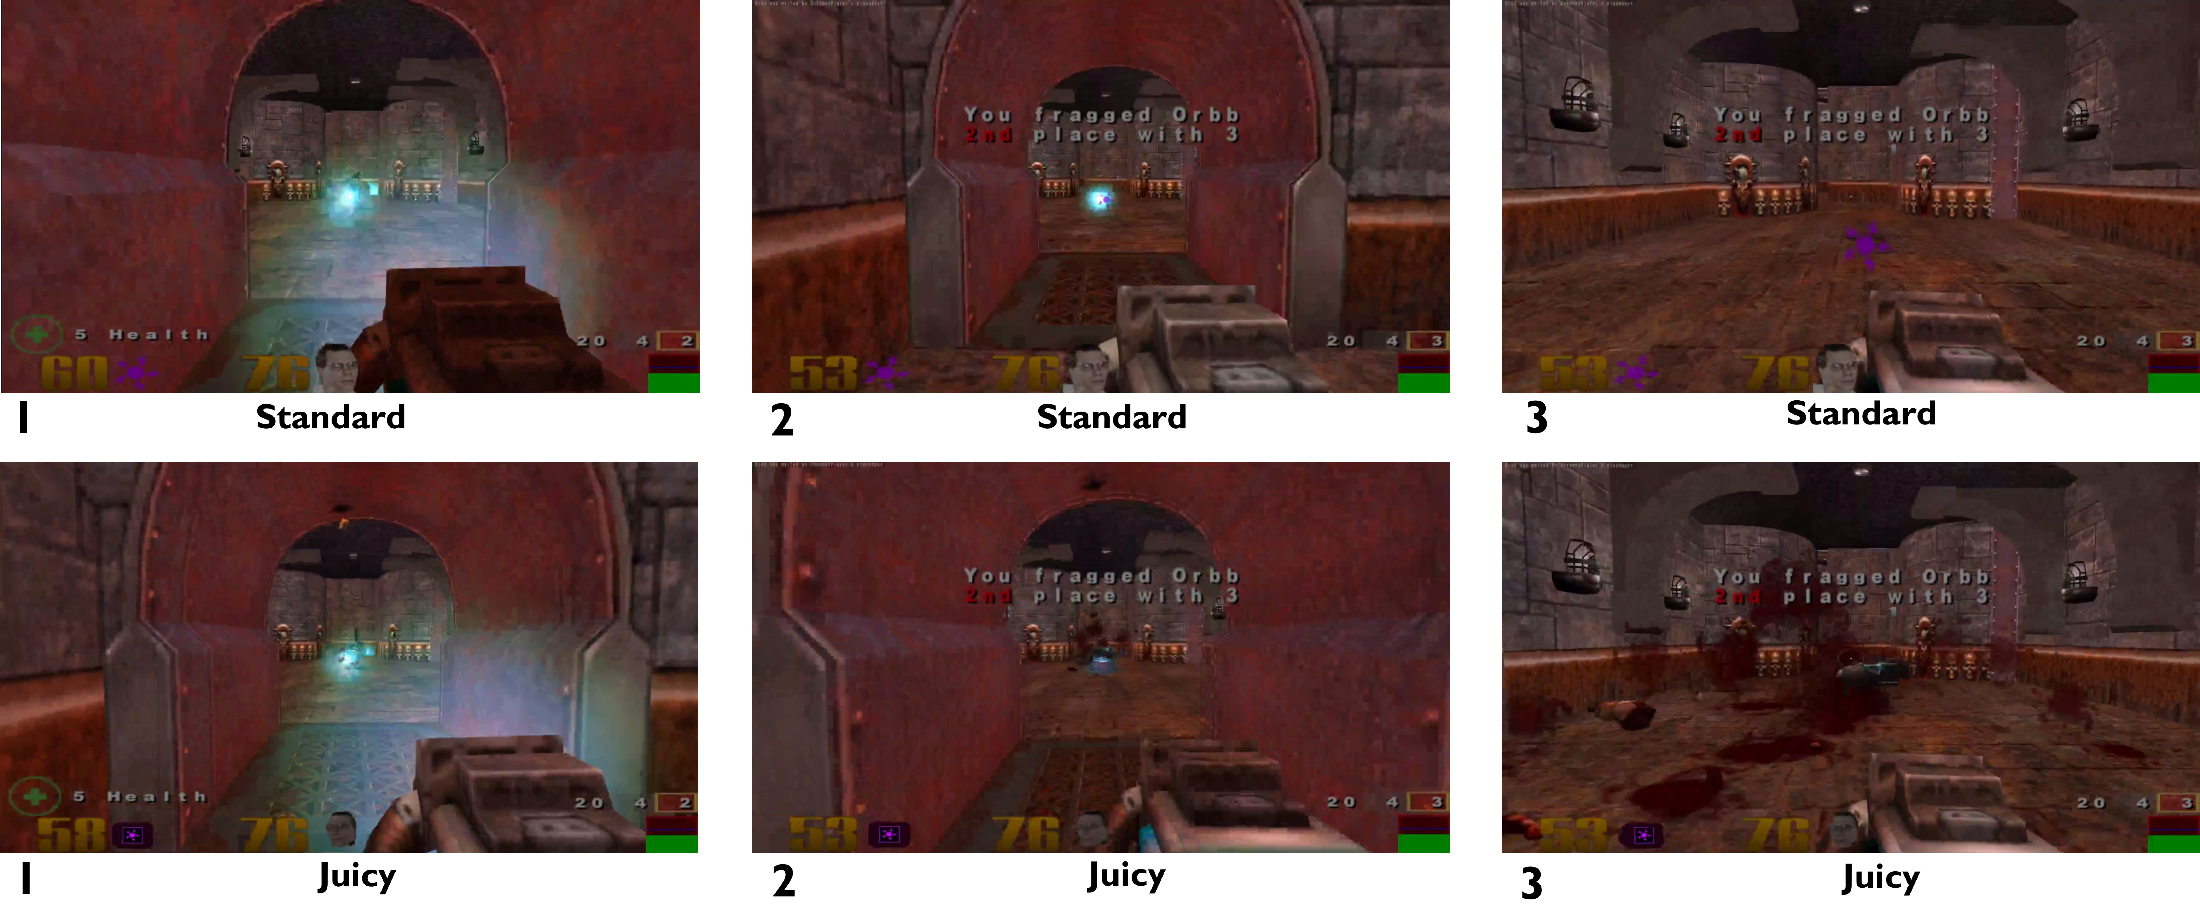
\includegraphics[width=\textwidth]{figures/Quake_Timeline.png}
	\caption{Presentation of gameplay in \textit{Quake 3} as the player shoots an opposing player (top row: standard version, bottom row: juicy version; see video figure for full overview of animation effects).}
	\label{figure:quaketimeline}
\end{figure*}

\subsection{Validation of Juiciness}
We validated the custom-built games, more specifically the non-juicy and juicy versions using the elements described above, to ensure that juicy versions contained suitable juicy elements, and that the standard versions did not (but could still be considered finished and polished games). To this end, we recruited four game designers who played through each version of Cuber and Dungeon Descent independently, and then applied the juicy framework \cite{hicks2018juicy}, reporting on whether the game met each of the framework's questions. Designers played each version of the game for 30 minutes, at which point they went through each question in the framework answering "yes" or "no", providing a rationale for their answers when needed. Using the framework, all four designers confirmed that the juicy version comprised appropriate juicy features in line with the framework and other work in this field, that the standard version did not, and that the differences between both versions were clear when compared directly.  
 
\section{UNDERSTANDING THE EFFECTS OF JUICINESS}
Here, we present two studies exploring the effects of Juiciness on players. We first give an overview of research questions, hypotheses, and measures. Second, we report findings from a study with 40 participants exploring the effects of juiciness in research games. Third, we replicate the first study with 32 participants who did not take part in the first study using a commercially available game that offers more depth in terms of gameplay.

\subsection{Research Question and Hypotheses}
Through our work, we aim to address the following three main research questions (RQs) concerned with the relationship of players and juiciness: 
\\\\
\textbf{RQ1:} Does juiciness improve player experience?
\\
Literature suggests that juiciness leads to improvements in player experience, often on the basis of improved visual appeal \cite{swink2008game,juul2010casual}. We therefore formulate the following hypotheses:
\\
\textit{H1a: Juiciness increases the aesthetic appeal of games.}
\\
\textit{H1b: Juiciness improves the overall player experience.}
\\
\\
\textbf{RQ2:} Does juiciness have an impact on player performance? 
\\
Previous work suggests that juiciness contributes to player competence \cite{deterding2015lens}. We are particularly interested to explore whether juiciness affects perceived competence or objective player performance; this led to the following hypotheses:
\\
\textit{H2a: Juiciness improves perceived competence.}
\\
\textit{H2b: Juiciness improves objective player performance.}
\\
\subsection{Measures}
We combined a number of measures to address the research questions.
\subsubsection{Questionnaires}
We include three questionnaires, two of which are validated. We use these to explore the impact of juiciness on players, along with an open-ended exit questionnaire that collects overall feedback including qualitative statements.
\\\\
\textbf{Player Experience.} To evaluate player experience, we include the Player Experience and Needs Satisfaction (PENS) questionnaire and the Player Experience Inventory (PXI). The PENS is validated and a de-facto standard in games research (e.g., see \cite{ang2017comparing}, \cite{hicks2015exploring} and \cite{bowey2015manipulating} for examples of its application in the CHI games research community). It builds on Self-Determination Theory \cite{ryan2000self,ryan2006motivational} and includes sub-scales for Competence, Autonomy, Presence, Relatedness, and Intuitive Controls. Participants are asked to rate statements such as "I feel competent at the game" on a 7-point Likert scale. The PXI is a novel tool for the assessment of player experience that makes a distinction between psychological and tangible factors \cite{vanden2016design}. The PXI contains sub-scales for Mastery, Curiosity, Immersion, Autonomy, Meaning, Clarity of Rules and Goals, Appeal, Challenge, Ease of Control, and Progress Feedback. Participants are asked to rate statements such as "I appreciated the aesthetics of the game" on a 7-point Likert scale. Internal consistence of the subscales was measured via Cronbach's Alpha (see Table \ref{table:GameTable}), all scales reached satisfactory levels except for PENS Relatedness which was dropped from the analysis.
\\\\
\textbf{Aesthetic Appeal.} To measure the aesthetic appeal in general and visual attractiveness of the games in particular, we adapted the AttrakDiff2 questionnaire \cite{hassenzahl2003attrakdiff}. The AttrakDiff2 is a validated measure that is commonly applied in user experience research (e.g., \cite{hassenzahl2006hedonic}); although it has not been used extensively in games. The questionnaire examines pragmatic and hedonistic qualities of interactive products using a semantic differential. Participants are given two verbal anchors such as "Ugly" and "Beautiful" at each end of a 7-point Likert scale. In addition to the hedonic and pragmatic dimensions it also has dimensions of beauty which explores the visual aesthetic appeal and goodness which covers the pleasure of use.
\\\\
\textbf{Direct Player Feedback.} We employed an exit questionnaire that asked participants about differences between conditions, ratings of subjective enjoyment on a 7-point Likert scale, and condition rankings in order of preference. We further solicited open-ended comments on player preferences along with the idea of juiciness.

\subsubsection{Game Metrics}
\textit{Dungeon Descent}, \textit{Cuber} and \textit{Quake 3} store a variety of game metrics in order to look at the effects of juicy design on performance and behaviour. For \textit{Dungeon Descent}, we recorded the score and combo multiplier, weapon accuracy, and levels cleared as performance metrics. Additionally, we recorded how many times the player performed actions such as jumping or attacking, and positional data to explore player behaviour. Performance metrics recorded for \textit{Cuber} include the score, lives lost, time spent per level, and levels cleared. For behavioural metrics we recorded positional data and the number of button presses. For the first-person shooter \textit{Quake 3}, we include player kills and deaths in analysis.

\subsection{Study 1: Juiciness in Research Games}
We present a within-subjects study exploring the effects of juiciness on player experience, performance and overall player perspectives using \textit{Cuber} and \textit{Dungeon Descent}.

\subsubsection{Participants and Procedure}
We recruited 40 participants (23 male, average age 26, SD=7.6) through word of mouth, mailing lists and, social media sites. When screening for visual impairments that might interfere with study participation, 2 participants reported colour vision deficiency, but later on indicated that they were able to discern juicy elements with no issues and were therefore retained in analysis. Of the participants, 28 were experienced players (more than 5 hours of regular gameplay per week); 6 were casual players (1-4 hours a week), and 6 were not actively playing games. 
\\\\
At the start of the study, each participant was given information on the study, and asked to provide informed consent. 
The study was split into four sequences consisting of one of the conditions (\textit{Standard, Juicy}) of \textit{Cuber} and \textit{Dungeon Descent}; counterbalanced using a Latin square to control for order effects). In each condition, participants were asked to play each of the game versions for at least 5 minutes but were permitted to play up to 10. After each condition, participants were asked to fill out the questionnaires on player experience, and aesthetic appeal. At the end of the study, participants were asked to complete the exit questionnaire which involved rating the enjoyment of each of the games and ranking them for preference. Additionally demographic information along with information on their gaming habits was recorded in this questionnaire. Finally, participants were given the opportunity to ask questions related to the study and research, and thanked for their participation. On average, sessions lasted about 75 minutes. The research protocol was approved by the ethics board at <removed for blind review>
\subsubsection{Data Analysis}
Quantitative data were analyzed in SPSS 22. We applied a two-way repeated measures ANOVA with Embellishment (\textit{Standard}, \textit{Juicy}) and Game (\textit{Cuber}, \textit{Dungeon Descent}) as within-subject factors for questionnaire data (PENS, PXI, and AttrakDiff2) and post-play enjoyment ratings. Pairwise comparisons were made with Bonferroni correction. Performance data were analyzed with paired-samples t-tests.
\subsubsection{Results}
The results section is organized according to our research questions. Quantitative findings are supplemented with qualitative participant feedback.

\begin{scriptsize}
\begin{table}[]
\caption{Player metrics that were stored based on the game}
\label{table:metrics}
\begin{tabular}{p{1.1cm}lp{1.1cm}p{1.1cm}l}
\hline
                         & \textbf{Metric}         & \textbf{Base}     & \textbf{Juicy}    & \textbf{P} \\ \hline
\textbf{Cuber}           & \textbf{Levels Cleared} & 4.5 (1.48)         & 4.45 (1.50)        & $p=.772$                  \\
                         & \textbf{Deaths}         & 10.30 (6.41)       & 9.22 (5.64)        & $p=.316$                  \\
                         & \textbf{Score}          & 3988.50 (1291.88)  & 3941.50 (1303.47)  & $p=.781$                  \\ \hline
\textbf{Dungeon Descent} & \textbf{Accuracy}       & 43.27 (0.13\%) & 44.41 (0.19\%) & $p=.670$                  \\
                         & \textbf{Kills}          & 49.45 (29.29)      & 50.77 (26.42)      & $p=.808$                  \\
                         & \textbf{Levels}         & 6.77 (3.33)        & 6.35 (2.42)        & $p=.494$                  \\
                         & \textbf{Deaths}         & 1.27 (1.03)        & 1.22 (0.86)        & $p=.785$                  \\
                         & \textbf{Score}          & 473,062 (621,307)  & 317,800 (371,073)  & $p=.206$                  \\ \hline
\textbf{Quake 3}         & \textbf{Kills}          & 50.65 (17.81)      & 52.06 (19.47)      & $p=.606$                  \\
                         & \textbf{Deaths}         & 11.28 (3.22)      & 12.65 (3.41)        & $p=.808$  
\end{tabular}
\end{table}
\end{scriptsize}

\textbf{RQ1: Does Juiciness Improve Player Experience?}
Juiciness does improve player experience in both research games in terms of visual appeal, and related constructs such as curiosity, immersion and meaning. However, it does not affect player experience in terms of needs satisfaction.

\textit{H1a: Juiciness increases the aesthetic appeal of games.} Our results support H1a, suggesting that juiciness increases the aesthetic and visual appeal of the two research games. Results for the AttrakDiff (see Tables \ref{table:GameTable} and \ref{table:PanasTable}) reveal a significant main effect of embellishment on the dimensions of hedonic identification (HQI) and stimulation (HQS), but no interaction between game and embellishment, suggesting that juiciness increased hedonic quality (with HQS referring perceived novelty and stimulation, and HQI referring to communicating identity) across conditions. However, for the items of Beauty and Goodness, there was no significant difference, suggesting juiciness does not improve the perceived beauty or pleasure of the game. The PXI revealed a significant main effect of juiciness on the dimension of audiovisual appeal, but no interaction between game and embellishment, suggesting that the concept improved player perceptions across games. Qualitative participant responses support the notion of juiciness improving the aesthetic appeal of games, e.g.,  one participant noting that juicy game versions "\textit{felt more immersive in the [juicy] version, and visually more appealing}" (P27).
%\begin{figure*}
%	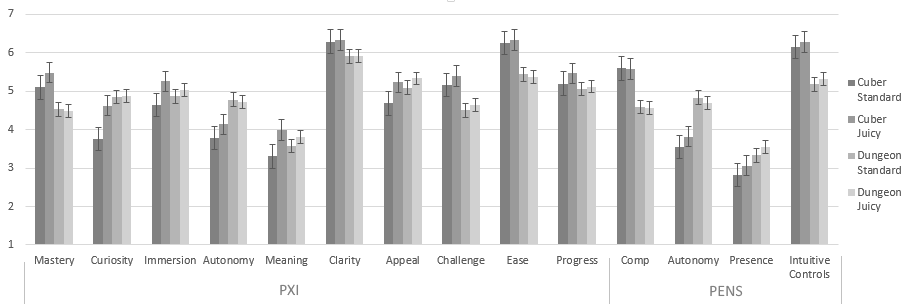
\includegraphics[width=\textwidth]{figures/PENS_PXI_Graph}
%	\caption{Mean values and SE for player experience according to the PXI and PENS Questionnaires, measured %on 7-point Likert scales (higher = better). Results demonstrate above-average player experience in both %games (see Table 2 for significant effects of game).}
%	\label{figure:PXIChart}
%\end{figure*}
\begin{table*}
  \caption{Means, Standard Deviation, Reliability, and F-scores split by game and condition for each dimension of PENS and PXI. * of Significance}
  \label{table:GameTable}
   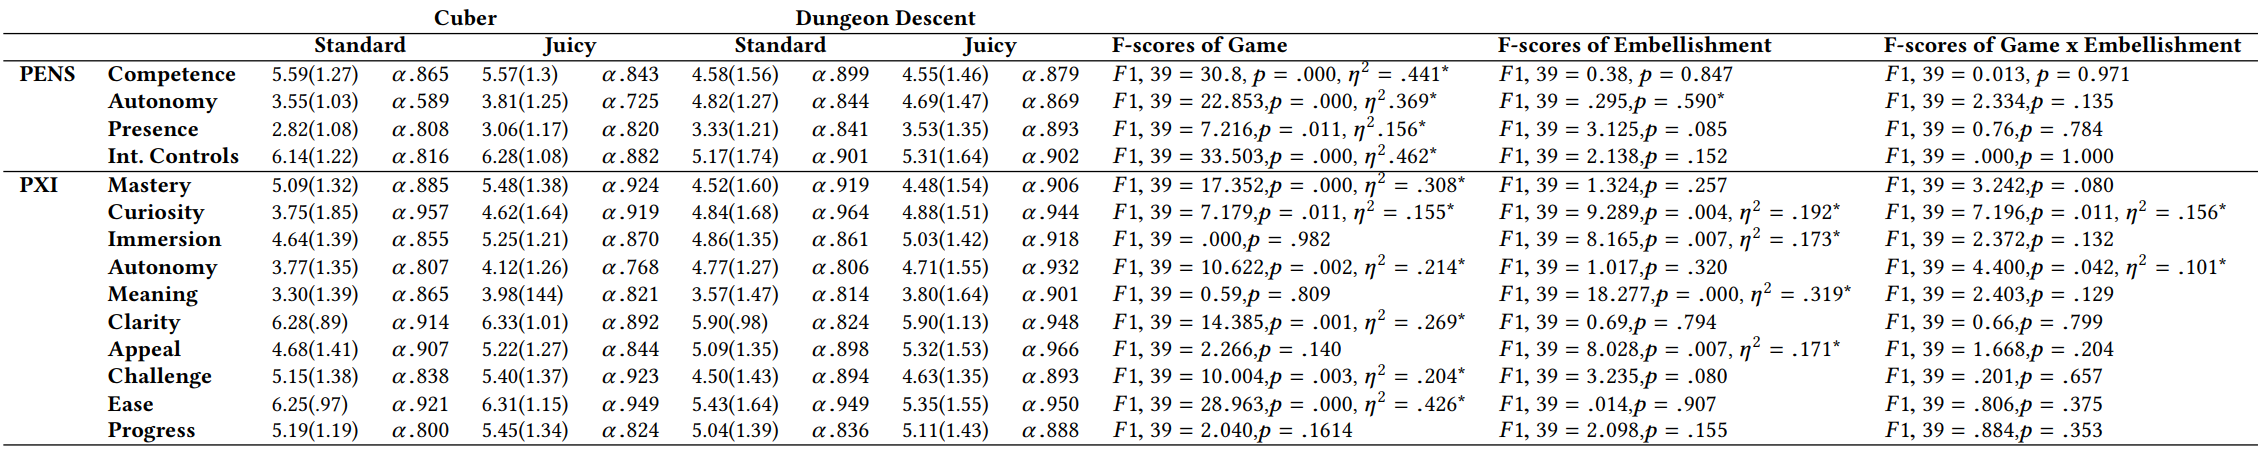
\includegraphics[width=\textwidth]{figures/Game_Exp_Table}
\end{table*}
\begin{table*}
  \caption{Means, Standard Deviation, Reliability, and F-scores split by game and condition for each dimension of AtrakDiff2. * of Significance}
  \label{table:PanasTable}
  	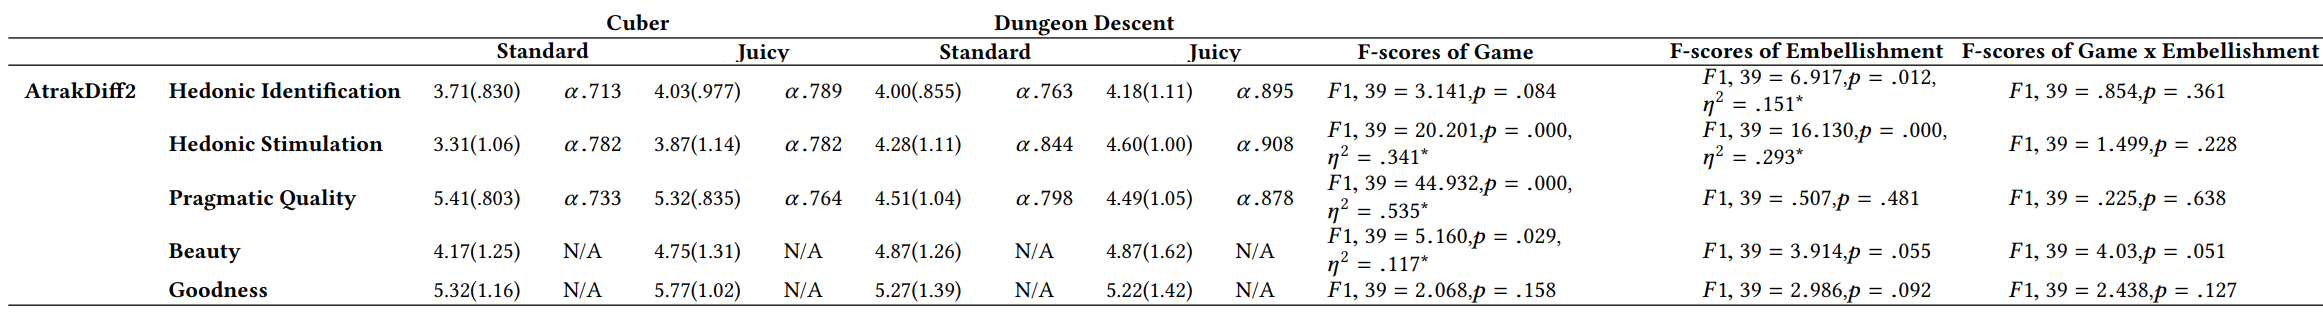
\includegraphics[width=\textwidth]{figures/PANAS_ATRAKDIFF2_Table}
\end{table*}
\\\\
\textit{H1b: Juiciness improves the overall player experience.}
Our results partially support this hypothesis with respect to the two research games. There were no significant main effects of juiciness on any of the scales of the PENS, and no interaction effects (see Table \ref{table:GameTable}), the PXI component of Autonomy also did not show a significant difference, suggesting that in this particular setting, juiciness does not contribute to the satisfaction of player needs as defined by Self-Determination Theory. However, the PXI revealed significant main effects of juiciness on the dimensions of Immersion, Meaning, Curiosity, and no interaction effects between game and visual embellishment. The effect of Curiosity needs to be interpreted in the light of the interaction between game and embellishment, suggesting that the impact in \textit{Cuber} was the driving element. These results support the hypothesis that juiciness does have an effect on some elements of player experience, particularly those directly relating to game visuals (e.g., immersion, or curiosity instilled by interesting visual effects). Qualitative participant responses also reflect differences in player experience, with participants expressing the juicy versions 'felt' better, e.g., "\textit{[...] the special effects on the enemies when they died and movement felt more real}" (P7). Participants also reflected on the changes to the experience juiciness provided "\textit{I preferred the second version (Juicy Cuber) because it just felt more engaging and interactive when playing.}" (P3). However, these results do not seem to affect overall enjoyment of the conditions, which all achieved similar ratings ($M_\text{Cuber Standard}=4.8$, $SD_{Cuber Standard}=1.771$,$M_\text{Cuber Juicy}=4.9$, $SD_{Cuber Juicy}=1.958$,$M_\text{Dungeon Standard}=4.95$, $SD_{Dungeon Standard}=1.518$, $M_\text{Dungeon Juicy}=5.07$, $SD_{Dungeon Juicy}=1.384$). There was no significant main effect of game $F_{1,39} = .198$, $p = .659$, $\eta^2=.005$, or embellishment $F_{1,39} = .552$, $p = .462$, $\eta^2=.014$, and no interaction between Game and Embellishment $F_{1,39} = .003$, $p = .957$, $\eta^2=.000$. 
\\\\
\textbf{RQ2: Does Juiciness Have an Impact on Player Performance?}
Our results do not support the idea that juiciness can be leveraged to improve player performance, or increase perceived competence in the two games. 
\\\\
\textit{H2a: Juiciness improves perceived competence.}
Our results do not support H2a. To explore changes in perceived competence, we analyzed relevant PENS and PXI dimensions (see Table \ref{table:GameTable}). For the Competence dimension of the PENS, there were no significant effects. For the PXI, we analyzed the dimensions of Mastery and Challenge, with no significant effects found. Interestingly, participant responses were ambivalent regarding the effects of juiciness in terms of performance. For example, one participant expressed higher levels of competence in the standard version, "\textit{the player controls were more to what I'm used to (not a lot of screen shake/head motion when attacking), which made it easier for me to control my character}" (P15), whereas another participant commented that "\textit{Juicy Cuber was slightly more difficult as the animations meant slightly more to focus on}" (P38), suggesting that the interpretation of the effects of elements of juicy design on perceived competence was highly individual. In this context, it is important to note that there were no significant differences in Ease of Use (PXI) or Intuitive Controls (PENS) between standard and embellished game versions, suggesting that the basic usability provided by both game versions was perceived as comparable (see Table \ref{table:GameTable}).
\\\\
\textit{H2b: Juiciness improves objective player performance.}
To measure whether the inclusion of juiciness had an effect on player performance in the two research games, we compared several metrics between the standard and embellished version of each game. For \textit{Cuber}, we compared the amount of levels cleared, amount of deaths, and score, finding no significant differences between any metrics (see Table \ref{table:metrics}). For \textit{Dungeon Descent}, we compared the amount of levels cleared, score, amount of deaths, kills, and accuracy. We found no significant differences between any of these metrics either (see Table \ref{table:metrics}). Therefore, our data does not support H2b. 

\begin{comment}
\afterpage{%
    \clearpage
    \thispagestyle{empty}

\begin{scriptsize}

\begin{sidewaystable}[h]
\vspace{2in}
	\caption{Means, Standard Deviation, Reliability, and Effects split by game and condition for each dimension. * represents significance}
\begin{tabular}{lllllllllllll}
              & \textbf{}              & \multicolumn{4}{c}{\textbf{Cuber}}                                         & \multicolumn{4}{c}{\textbf{Dungeon Descent}}                               &                              &                                  &                               \\ \hline
\textbf{}     & \textbf{}              & \multicolumn{2}{c}{\textbf{Standard}} & \multicolumn{2}{c}{\textbf{Juicy}} & \multicolumn{2}{c}{\textbf{Standard}} & \multicolumn{2}{c}{\textbf{Juicy}} & \textbf{F-scores of Game}      & \textbf{F-scores of Embellishment} & \textbf{F-scores of Game x Embellishment} \\ \hline
\textbf{PENS} & \textbf{Competence}    & 5.59(1.27)           & $\alpha.865$           & 5.57(1.3)           & $\alpha.843$         & 4.58(1.56)           & $\alpha.899$           & 4.55(1.46)          & $\alpha.879$         & $F{1,39}=30.8$, $p=.000$, $\eta^2=.441$*  & $F{1,39}=0.38$, $p=0.847$             & $F{1,39}=0.013$, $p=0.971$          \\
\textbf{}     & \textbf{Autonomy}      & 3.55(1.03)           & $\alpha.589$           & 3.81(1.25)          & $\alpha.725$         & 4.82(1.27)           & $\alpha.844$           & 4.69(1.47)          & $\alpha.869$         & $F{1,39}=22.853$,$p=.000$, $\eta^2.369$* & $F{1,39}=.295$,$p=.590$*                & $F{1,39}=2.334$,$p=.135$            \\
\textbf{}     & \textbf{Presence}      & 2.82(1.08)           & $\alpha.808$           & 3.06(1.17)          & $\alpha.820$         & 3.33(1.21)           & $\alpha.841$           & 3.53(1.35)          & $\alpha.893$         & $F{1,39}=7.216$,$p=.011$, $\eta^2.156$*  & $F{1,39}=3.125$,$p=.085$               & $F{1,39}=0.76$,$p=.784$             \\
\textbf{}     & \textbf{Int. Controls} & 6.14(1.22)           & $\alpha.816$           & 6.28(1.08)          & $\alpha.882$         & 5.17(1.74)           & $\alpha.901$           & 5.31(1.64)          & $\alpha.902$         & $F{1,39}=33.503$,$p=.000$, $\eta^2.462$* & $F{1,39}=2.138$,$p=.152$               & $F{1,39}=.000$,$p=1.000$            \\ \hline
\textbf{PXI}  & \textbf{Mastery}   & 5.09(1.32)           & $\alpha.885$           & 5.48(1.38)          & $\alpha.924$         & 4.52(1.60)           & $\alpha.919$           & 4.48(1.54)          & $\alpha.906$         & $F{1,39}=17.352$,$p=.000$, $\eta^2=.308$* & $F{1,39}=1.324$,$p=.257$               & $F{1,39}=3.242$,$p=.080$            \\
\textbf{}     & \textbf{Curiosity} & 3.75(1.85)           & $\alpha.957$           & 4.62(1.64)          & $\alpha.919$         & 4.84(1.68)           & $\alpha.964$           & 4.88(1.51)          & $\alpha.944$         & $F{1,39}=7.179$,$p=.011$, $\eta^2=.155$*  & $F{1,39}=9.289$,$p=.004$, $\eta^2=.192$*      & $F{1,39}=7.196$,$p=.011$, $\eta^2=.156$*   \\
\textbf{}     & \textbf{Immersion} & 4.64(1.39)           & $\alpha.855$           & 5.25(1.21)          & $\alpha.870$         & 4.86(1.35)           & $\alpha.861$           & 5.03(1.42)          & $\alpha.918$         & $F{1,39}=.000$,$p=.982$            & $F{1,39}=8.165$,$p=.007$, $\eta^2=.173$*      & $F{1,39}=2.372$,$p=.132$            \\
\textbf{}     & \textbf{Autonomy}  & 3.77(1.35)           & $\alpha.807$           & 4.12(1.26)          & $\alpha.768$         & 4.77(1.27)           & $\alpha.806$           & 4.71(1.55)          & $\alpha.932$         & $F{1,39}=10.622$,$p=.002$, $\eta^2=.214$* & $F{1,39}=1.017$,$p=.320$               & $F{1,39}=4.400$,$p=.042$, $\eta^2=.101$*   \\
\textbf{}     & \textbf{Meaning}   & 3.30(1.39)           & $\alpha.865$           & 3.98(144)           & $\alpha.821$         & 3.57(1.47)           & $\alpha.814$           & 3.80(1.64)          & $\alpha.901$         & $F{1,39}=0.59$,$p=.809$            & $F{1,39}=18.277$,$p=.000$, $\eta^2=.319$*     & $F{1,39}=2.403$,$p=.129$            \\
\textbf{}     & \textbf{Clarity}   & 6.28(.89)            & $\alpha.914$           & 6.33(1.01)          & $\alpha.892$         & 5.90(.98)            & $\alpha.824$           & 5.90(1.13)          & $\alpha.948$         & $F{1,39}=14.385$,$p=.001$, $\eta^2=.269$* & $F{1,39}=0.69$,$p=.794$                & $F{1,39}=0.66$,$p=.799$             \\
\textbf{}     & \textbf{Appeal}    & 4.68(1.41)           & $\alpha.907$           & 5.22(1.27)          & $\alpha.844$         & 5.09(1.35)           & $\alpha.898$           & 5.32(1.53)          & $\alpha.966$         & $F{1,39}=2.266$,$p=.140$           & $F{1,39}=8.028$,$p=.007$, $\eta^2=.171$*      & $F{1,39}=1.668$,$p=.204$            \\
\textbf{}     & \textbf{Challenge} & 5.15(1.38)           & $\alpha.838$           & 5.40(1.37)          & $\alpha.923$         & 4.50(1.43)           & $\alpha.894$           & 4.63(1.35)          & $\alpha.893$         & $F{1,39}=10.004$,$p=.003$, $\eta^2=.204$* & $F{1,39}=3.235$,$p=.080$               & $F{1,39}=.201$,$p=.657$             \\
\textbf{}     & \textbf{Ease}      & 6.25(.97)            & $\alpha.921$           & 6.31(1.15)          & $\alpha.949$         & 5.43(1.64)           & $\alpha.949$           & 5.35(1.55)          & $\alpha.950$         & $F{1,39}=28.963$,$p=.000$, $\eta^2=.426$* & $F{1,39}=.014$,$p=.907$                & $F{1,39}=.806$,$p=.375$             \\
\textbf{}     & \textbf{Progress}  & 5.19(1.19)           & $\alpha.800$           & 5.45(1.34)          & $\alpha.824$         & 5.04(1.39)           & $\alpha.836$           & 5.11(1.43)          & $\alpha.888$         & $F{1,39}=2.040$,$p=.1614$           & $F{1,39}=2.098$,$p=.155$               & $F{1,39}=.884$,$p=.353$             \\ \hline
\end{tabular}
\end{sidewaystable}
\end{scriptsize}

\begin{scriptsize}
\begin{sidewaystable}[h]
\vspace{2in}
	\caption{Means, Standard Deviation, Reliability, and Effects split by game and condition for each dimension. * represents significance}
\begin{tabular}{p{1cm}p{1cm}llllllllllll}
                    & \textbf{}                       & \multicolumn{4}{c}{\textbf{Cuber}}                                         & \multicolumn{4}{c}{\textbf{Dungeon Descent}}                               &                                                                        &                                                                        &                               \\ \hline
\textbf{}           & \textbf{}                       & \multicolumn{2}{c}{\textbf{Standard}} & \multicolumn{2}{c}{\textbf{Juicy}} & \multicolumn{2}{c}{\textbf{Standard}} & \multicolumn{2}{c}{\textbf{Juicy}} & \textbf{F-scores of Game}                                                & \textbf{F-scores of Embellishment}                                       & \textbf{F-scores of Game x Embellishment} \\ \hline
\textbf{PANAS}      & \textbf{Positive Affect}        & 26.32(9.73)           & $\alpha.919$          & 27.55(9.74)         & $\alpha.885$         & 28.67(8.48)           & $\alpha.913$          & 28.27(8.71)         & $\alpha.927$         & $F{1,39}=1.590$,$p=.215$                                                     & $F{1,39}=.295$,$p=.590$                                                      & $F{1,39}=1.396$,$p=.245$            \\
\textbf{}           & \textbf{Negative Affect}        & 13.15(4.75)           & $\alpha.657$          & 12.40(4.59)         & $\alpha.880$         & 19.10(19.26)          & $\alpha.771$          & 14.87(6.66)         & $\alpha.771$         & $F{1,39}=6.264$,$p=.017$, $\eta^2=.138$*                                            & $F{1,39}=2.692$,$p=.075$                                                     & $F{1,39}=3.342$,$p=.079$            \\ \hline
\textbf{AtrakDiff2} & \textbf{Hedonic Identification} & 3.71(.830)            & $\alpha.713$          & 4.03(.977)          & $\alpha.789$         & 4.00(.855)            & $\alpha.763$          & 4.18(1.11)          & $\alpha.895$         & $F{1,39}=3.141$,$p=.084$                                                     & \begin{tabular}[c]{@{}l@{}}$F{1,39}=6.917$,$p=.012$,\\ $\eta^2=.151$*\end{tabular}  & $F{1,39}=.854$,$p=.361$             \\
\textbf{}           & \textbf{Hedonic Stimulation}    & 3.31(1.06)            & $\alpha.782$          & 3.87(1.14)          & $\alpha.782$         & 4.28(1.11)            & $\alpha.844$          & 4.60(1.00)          & $\alpha.908$         & \begin{tabular}[c]{@{}l@{}}$F{1,39}=20.201$,$p=.000$,\\ $\eta^2=.341$*\end{tabular} & \begin{tabular}[c]{@{}l@{}}$F{1,39}=16.130$,$p=.000$,\\ $\eta^2=.293$*\end{tabular} & $F{1,39}=1.499$,$p=.228$            \\
\textbf{}           & \textbf{Pragmatic Quality}      & 5.41(.803)            & $\alpha.733$          & 5.32(.835)          & $\alpha.764$         & 4.51(1.04)            & $\alpha.798$          & 4.49(1.05)          & $\alpha.878$         & \begin{tabular}[c]{@{}l@{}}$F{1,39}=44.932$,$p=.000$,\\ $\eta^2=.535$*\end{tabular} & $F{1,39}=.507$,$p=.481$                                                      & $F{1,39}=.225$,$p=.638$             \\
\textbf{}           & \textbf{Beauty}                 & 4.17(1.25)            & N/A          & 4.75(1.31)          & N/A         & 4.87(1.26)            & N/A          & 4.87(1.62)          & N/A         & \begin{tabular}[c]{@{}l@{}}$F{1,39}=5.160$,$p=.029$,\\ $\eta^2=.117$*\end{tabular}  & $F{1,39}=3.914$,$p=.055$                                                     & $F{1,39}=4.03$,$p=.051$             \\
\textbf{}           & \textbf{Goodness}               & 5.32(1.16)            & N/A          & 5.77(1.02)          & N/A         & 5.27(1.39)            & N/A          & 5.22(1.42)          & N/A        & $F{1,39}=2.068$,$p=.158$                                                     & $F{1,39}=2.986$,$p=.092$                                                     & $F{1,39}=2.438$,$p=.127$            \\ \hline
\end{tabular}
\end{sidewaystable}
\end{scriptsize}


\clearpage
}
\end{comment}

\subsection{Study 2: Juiciness in Commercial Games}
In order to strengthen our findings and explore generalizability beyond research games, we present a replication of the first study, using a within-subjects design that examines the effects of juiciness in the first-person shooter \textit{Quake 3}.

\subsubsection{Game Description: Quake 3 Arena}
\textit{Quake 3 Arena} is a commercial death match first person shooter that was first released in 1999 \cite{quake3arena:pc}, and re-released in 2010 as online version under the name \textit{Quake Live} \cite{quake3live:pc}. Today, the game is available via Steam and is still actively played across the world \cite{Quake3Stats}. The game is geared toward competition and does not feature extensive narrative elements, the goal of the game simply is to try and defeat - or \textit{frag} - as many opponents as possible (see video figure). To this end, the player controls an avatar in an arena, and must move around to collect weapons and power-ups while attempting to kill opposing players (AI-controlled in single player mode, or human competitors). If the player is killed before the end of the level, they respawn at one of several predefined spawn points in the level, but lose all weapons and power-ups. At the end of each level (determined either through frag or time limit), an overview of scores is presented to players. The game features a range of competition modes (e.g., duel, free for all, team deathmatch). In our study, we employ single player competition against several AI-controlled opponents at medium difficulty to provide a comparable experience to all participants.
\\\\
\texti{Quake 3} has previously been leveraged as research tool and has previously been leveraged in research \cite{Bakaoukas2016}; we selected the game because it offers off-the-shelf customization options that fall in line with our definition of Juiciness. Additionally, the game strongly emphasizes competition and performance through these elements of Juicy Design while offering straightforward and engaging gameplay, making it a suitable candidate for our research largely in line with recommendations for selection of games for research studies \cite{Tyack2018}.
\subsubsection{Juicy Elements}
 Similar to our previous approach, the configuration of juicy elements for the juicy version of the game was done following guidelines laid out by \cite{deterding2015lens,hicks2018juicy,juul2016good}. In the juicy version, enemies emit an additional \textbf{particle effect} resembling blood when hit by the player; when killed they explode into a fountain of blood and gore. Additionally, the juicy version also includes added \textbf{particle and trail effects} for weapons. These three elements in particular are in line with those implemented in \textit{Dungeon Descent}. Finally, collectable items (e.g., power-ups, weapons) are integrated into the environment as 3D objects with \textbf{subtle animations} rather than simple 2D icons. For a comparison of base and juicy versions, please see Figure \ref{figure:quaketimeline} or consult the video figure.
 
 \subsubsection{Participants and Procedure}
We recruited 32 participants (21 male, average age 23, SD=3.58) through word of mouth, mailing lists, and social media sites. When screening for visual impairments that might interfere with study participation, 2 participants reported colour vision deficiency, but later on indicated that they were able to discern juicy elements with no issues and were therefore retained in analysis. Of the participants, 26 were experienced players (more than 5 hours of regular gameplay per week); 4 were casual players (1-4 hours a week), and 2 were not actively playing games. 
\\\\
At the start of the study, each participant was given information on the study, and asked to provide informed consent. 
The study was split into two sequences consisting of one of the conditions (\textit{Standard, Juicy}) of \textit{Quake 3}, counterbalanced to control for order effects). Participants were asked to play each of the game versions for 9 minutes broken into 3 rounds of 3 minutes. After each condition, participants were asked to fill out the questionnaires on player experience, and aesthetic appeal. At the end of the study, participants were asked to complete the exit questionnaire which involved rating the enjoyment of each of the game versions and ranking them for preference. Additionally demographic information along with information on their gaming habits was recorded in this questionnaire. Finally, participants were given the opportunity to ask questions related to the study and research, and thanked for their participation. On average, sessions lasted about 45 minutes. The research protocol was approved by the ethics board at <removed for blind review>
\subsubsection{Data Analysis}
Quantitative data were analyzed in SPSS 22. We applied paired-samples t-tests with Embellishment (\textit{Standard}, \textit{Juicy}) as within-subject factors for questionnaire data (PENS, PXI, and AttrakDiff2), post-play enjoyment ratings, and performance data.
\subsubsection{Results}
Similar to the first study, we organize the results by research questions, and supplement quantitative findings with qualitative participant feedback.
\\\\
\textbf{RQ1: Does Juiciness improve player experience?} Juiciness improves player experience in \textit{Quake 3}, with the juicy version of the game receiving significantly higher ratings for visual appeal, curiosity, and immersion (see Table \ref{table:QuakeTable}; mirroring findings of the first study). However, our results further suggest that Juiciness also positively influences player experience with respect to need satisfaction, suggesting that juicy elements included in \textit{Quake 3} had different effects than those employed in the first study.
\\\\
\textit{H1a: Juiciness increases the aesthetic appeal of games.} Our results support H1a, suggesting that juiciness has a positive increase on the aesthetic and visual appeal of games. Results from the AttrakDiff2 reveal a significant main effect of embellishment on the hedonic identification (HQI) and stimulation (HQS), suggesting that juiciness increased hedonic quality. A significant effect was also found for both the beauty and goodness dimensions, suggesting that juiciness improved the perceived beauty and pleasure of the game. There was no significant effect of the pragmatic quality dimension which could suggest that juiciness has no effect on the perceived practicality of a game. The PXI revealed a significant main effect of juiciness on the audiovisual appeal dimension, suggesting again that the juicy effects enhanced the perceived visual appeal of the game. XXX QUAL SENTENCE HERE XXX 
\\\\
\textit{H1b: Juiciness improves the overall player experience.} The results partially support this hypothesis. There was a significant effect of juiciness in the competence scale of the PENS questionnaire. This suggests that the juiciness increased players perceived competence at meeting the games challenges. There was also a significant effect of juiciness for the PENS scale of presence suggesting that the juicy effects present in that condition increased the players perceived feeling of being there and in the moment. 
\\\\
\textbf{RQ2: Does Juiciness have an impact on player performance?}
Our results show that Juiciness positively influenced perceived competence, but that objective player performance remained unchanged.
\\\\
\textit{H2a: Juiciness improves perceived competence.} The results suggest that the juicy version of \textit{Quake 3} significantly increased perceived competence. For the PENS questionnaire, we analyzed the dimension Competence; the result was also reflected in the associated PXI dimension of Mastery, while not affecting Challenge (see Table \ref{table:QuakeTable}). Similar to the previous study qualitative player feedback revealed more nuanced perspectives. [Insert relevant quotes here.] Again, we did not find significant differences in Ease of Use (PXI) or Intuitive Controls (PENS) between the standard and embellished version of the game, suggesting comparable usability. Likewise, there was no significant difference in the PXI dimensions of Progress Feedback and Clarity of Goals and Rules, suggesting that standard and juicy versions of the game were comparable in terms of the basic information that they provide to players. 
\\\\
\textit{H2b: Juiciness improves objective player performance.}
XXX


\begin{scriptsize}
\begin{sidewaystable}
\caption{Means, Standard Deviation, Reliability, and F-scores for each dimension of PENS, PXI and AttrakDiff2. * of Significance}
  \label{table:QuakeTable}
\begin{tabular}{p{1.1cm}p{1.1cm}p{1.1cm}llll}
\hline
                    &                                 & \multicolumn{2}{c}{\textbf{Standard}} & \multicolumn{2}{c}{\textbf{Juicy}} & \textbf{F-Scores of Embellishment} \\ \hline
\textbf{PENS}       & \textbf{Competence}             & 5.22(.78)            & $\alpha0.219$          & 5.57(.82)          & $\alpha0.505$         & $F{1,31} = 5.83$, $p = .022$, $\eta^2=.158$*   \\
\textbf{}           & \textbf{Autonomy}               & 4.67(1.05)           & $\alpha0.798$          & 4.94(1.12)         & $\alpha0.696$         & $F{1,31} = 2.96$, $p = .095$             \\
\textbf{}           & \textbf{Relatedness}            & 2.41(1.35)           & $\alpha0.788$          & 2.21(1.08)         & $\alpha0.567$         & $F{1,31} = 1.36$, $p = .251$             \\
\textbf{}           & \textbf{Presence}               & 3.16(1.26)           & $\alpha0.889$          & 3.43(1.26)         & $\alpha0.85$          & $F{1,31} = 4.94$, $p = .034$, $\eta^2=.138$*   \\
\textbf{}           & \textbf{Int. Controls}          & 6.31(.68)            & $\alpha0.641$          & 6.43(.74)          & $\alpha0.825$         & $F{1,31} = .94$, $p = .338$              \\ \hline
\textbf{PXI}        & \textbf{Mastery}                & 5.43(.98)            & $\alpha0.685$          & 5.78(.91)          & $\alpha0.817$         & $F{1,31} = 6.26$, $p = .018$, $\eta^2=.168$*   \\
\textbf{}           & \textbf{Curiosity}              & 3.74(1.50)           & $\alpha0.883$          & 4.08(1.49)         & $\alpha0.81$          & $F{1,31} = 4.89$, $p = .035$, $\eta^2=.136$*   \\
\textbf{}           & \textbf{Immersion}              & 5.39(1.33)           & $\alpha0.902$          & 5.86(1.06)         & $\alpha0.843$         & $F{1,31} = 7.59$, $p = .010$, $\eta^2=.197$*   \\
\textbf{}           & \textbf{Autonomy}               & 4.98(1.59)           & $\alpha0.947$          & 5.43(1.16)         & $\alpha0.857$         & $F{1,31} = 4.17$, $p = .050$, $\eta^2=.119$*   \\
\textbf{}           & \textbf{Meaning}                & 4.13(1.30)           & $\alpha0.844$          & 4.42(1.20)         & $\alpha0.809$         & $F{1,31} = 2.33$, $p = .137$, $\eta^2=.137$*   \\
\textbf{}           & \textbf{Clarity}                & 6.68(.44)            & $\alpha0.671$          & 6.76(.44)          & $\alpha0.845$         & $F{1,31} = 1.44$, $p = .238$             \\
\textbf{}           & \textbf{Appeal}                 & 4.41(1.59)           & $\alpha0.911$          & 5.04(1.49)         & $\alpha0.917$         & $F{1,31} = 9.59$, $p = .004$, $\eta^2=.236$*   \\
\textbf{}           & \textbf{Challenge}              & 4.41(1.81)           & $\alpha0.928$          & 4.66(1.66)         & $\alpha0.878$         & $F{1,31} = .626$, $p = .435$             \\
\textbf{}           & \textbf{Ease}                   & 6.38(.58)            & $\alpha0.683$         & 6.39(.67)          & $\alpha0.576$         & $F{1,31} = .006$, $p = .940$             \\
\textbf{}           & \textbf{Progress}               & 6.11(1.00)           & $\alpha0.831$          & 6.27(.97)          & $\alpha0.761$         & $F{1,31} = 2.05$, $p = .162$             \\
\textbf{AtrakDiff2} & \textbf{Hedonic Identification} & 4.09(.83)            & $\alpha0.742$          & 4.53(.72)          & $\alpha0.586$         & $F{1,31} = 12.81$, $p = .001$, $\eta^2=.293$*  \\ \hline
\textbf{}           & \textbf{Hedonic Stimulation}    & 3.91(.81)            & $\alpha0.714$          & 4.25(.94)          & $\alpha0.746$         & $F{1,31} = 7.33$, $p = .011$, $\eta^2=.191$*   \\
\textbf{}           & \textbf{Pragmatic Quality}      & 4.92(1.06)           & $\alpha0.838$          & 5.16(.75)          & $\alpha0.642$         & $F{1,31} = 2.47$, $p = .126$             \\
\textbf{}           & \textbf{Beauty}                 & 3.56(1.24)           & N/A            & 4.34(1.53)         & N/A           & $F{1,31} = 13.92$, $p = .001$, $\eta^2=.310$*  \\
\textbf{}           & \textbf{Goodness}               & 5.18(1.42)           & N/A            & 6.03(.86)          & N/A           & $F{1,31} = 10.35$, $p = .003$, $\eta^2=.250$*  \\ \hline

\end{tabular}
\end{sidewaystable}
\end{scriptsize}

\subsection{Summary of Findings}
Our results show that Juiciness improves player experience (\textbf{RQ1}) across games, contributing to the perceived visual appeal of \textit{Cuber}, \textit{Dungeon Descent} and \textit{Quake 3} alike (\textit{H1a}). However, the effects of Juiciness on other elements that contribute to overall player experience (\textit{H1b}) needs to viewed in a more nuanced light: while the design strategy improved player immersion in both research games and the commercially available product, perceived player competence was only improved through the juicy elements integrated in \textit{Quake 3}, while the dimension of meaning was only impacted in the research games. Considering player performance, Juiciness did not improve objective indicators of success in any game; because perceived player performance (\textit{H2a}) was only affected in the commercial setting, we conclude that Juiciness does not contribute to player performance under all circumstances (\textbf{RQ2}), and that its integration requires further reflection if the intention is to improve satisfaction of psychological player needs.
\section{Discussion}
This paper explores visual embellishments - termed juiciness in games through two studies, first examining the first-person shooter \texit{Dungeon Descent} and the casual game \textit{Cuber}, and then focusing on the commercially available first-person shooter \textit{Quake 3}. Our findings show that juicy elements such as particle effects or animations have an impact on the aesthetic appeal of games, extending to curiosity and immersion experienced by players. However, our findings suggest that VEs only affect the satisfaction of basic psychological needs (e.g., competence and autonomy) under certain circumstances, and have no implications for player performance. Here, we discuss the implications of our findings with focus on the impact of juiciness on players, we present updated considerations for juicy design, and reflect on the implications of our results for the role of players as individuals with psychological needs and consumers of games.

\subsection{The Impact of Juiciness on Players}
Here, we discuss the results in the context of player experience, and we share implications for design that stem from our work.
\subsubsection{Effects of Juiciness on Player Experience and Performance}
Our results show that juicy design elements improve the visual appeal of a game, and contribute to curiosity experienced by players (e.g., contributing to the player's desire to explore a virtual world) by adding visual interest, suggesting that the design strategy has tangible benefits for players. Our findings further suggest that juicy design facilitates more immersive experiences, suggesting that VEs help players to become more engulfed in an experience, which could be leveraged to increase engagement or pique initial interest. However, our results demonstrate that juiciness only had effects on dimensions of the player experience that are linked with the satisfaction of psychological needs formulated within Self-Determination Theory (here: PENS competence and PXI mastery) in the commercially available game \textit{Quake 3}. We hypothesize that this effect is a result of careful design of juicy elements that have implications for player competence: the realistic display of blood on injury, and exaggerated amount of blood and gore on death of an opponent (also see Figure XX) leveraged in the game effectively reinforced the notion of success, while similar but more simplistic features in Dungeon Descent (flashing enemies on injury, stylized explosion on death - see video figure) did not achieve the same effect. This would imply that Juiciness needs to be designed with great care if the goal is to increase satisfaction of psychological needs through play: rather than introducing a wide range of general or abstract embellishments, the targeted use of realistic and contextually relevant VEs directly associated with indicators of player performance could offer tangible benefits for player experience. In this context, it is important to note that Juiciness did not impact objective player performance in any setting, which is in line with Juul's initial research into the effects of juiciness on players \cite{juul2016good}).

\subsubsection{Effects of Individual Elements and the Perceived Whole} While the overall picture of the effects of Juiciness was clear, qualitative feedback suggested individual instances of players who only appreciated certain aspects of Juiciness, but not others (e.g., screen shake in Dungeon Descent, item representation in Quake 3), suggesting that juicy elements either need to be assessed individually to ensure they contribute to player experience, or should be implemented in a way that allows players to toggle undesired effects. At the same time, feedback also shows many instances where a positive experience on the basis of Juiciness emerged from the overall impression of the game (with players being unable to point out specific elements of juicy design). This supports the 'intangible' nature of the phenomenon previously discussed, suggesting that positive effects stem from the combination of multiple elements that contribute to a more positive play experience.

\subsection{Understanding Players as Individuals With Various Needs}
Recent efforts in games research overwhelmingly focus on players as individuals with psychological needs through the lens of Self-Determination Theory (e.g., \cite{JOHNSON2016805,vella2017motivating}). Our results suggest that a broader perspective is required to explain the high-level effects of Juiciness. Here, approaches such as Uses and Gratifications theory could offer further insights: The theory assumes that individuals consume media with the goal of 'gratifying' certain needs \cite{lin1999uses,ruggiero2000uses}. Six gratifications have been associated with play: competition, challenge, social interaction, diversion, fantasy, and arousal \cite{sherry2006video}. The dimension of fantasy in particular - getting deeply involved in a virtual environment - relates to some of our findings, where Juiciness contributed to players' desire to explore the games (curiosity), and helped them have more engaging experiences (immersion). This suggests that Juiciness can help satisfy player needs related to media consumption, extending beyond the basic psychological needs as stipulated by Self-Determination Theory \cite{przybylski2010motivational}.
\subsection{Relevance of Our Findings for Game Development}
The effects of Juiciness have implications for both commercial game development, and the creation of games as research tools. From a commercial perspective, our findings suggest that elements of juicy design are important contributors to the overall aesthetic perception of a game, serving as an indicator of quality and polish that players leverage to assess the quality of a game. This ties back to the role of players as consumers: if they are given a choice between different products, market research suggests that graphical quality plays an important role \cite{usher_2014}; likewise, our findings highlight that players felt the juicy versions provided a more polished experience, or, as one participant put it, \textit{"I think the extra feedback given just made the game look nicer and more professional.}". The importance of visual appeal and first impressions is also backed by research in other fields, e.g., readers judging books by their covers \cite{yampbell2005judging}, or visitors forming an opinion of the visual appeal of websites within the blink of an eye \cite{lindgaard2006attention}. At the same time, the absence of significant effects of juiciness on main elements of player experience in research games (most importantly, autonomy along with competence) but presence in the commercially available product (increased perceived competence and mastery) has implications for the development of games as research tools: many implementations are visually simplistic (e.g., see \cite{brezinka2008treasure, laneau2005flexible, peddycord2017using}). Our findings suggest that this strategy needs to be applied with care depending on the experience the research tool is intended to invoke. Additionally, our findings suggest that researchers need to understand limitations that the impact of juiciness on visual appeal, curiosity and immersion imposes in research settings.
\section{Limitations and Future Work}
There are limitations to the work presented in this paper that need to be considered when interpreting our findings. Most importantly, our study only explored effects of visual juiciness; future work should also consider the impact of sound and music. Likewise, studying a broader range of game genres (e.g., real-time strategy, or sports games), further study of the impact of level of complexity (i.e., casual games and other games with a limited number of core mechanics versus more complex approaches such as sandbox-style games), and the study of juiciness in relationship with graphical realism (e.g., its impact in abstract versus photorealistic game worlds) would be beneficial. Future work should also explore effects in a real-world setting, and consider in-the-wild deployment of games to evaluate the long-term impact on player engagement. In terms of sampling, participants in our study particularly in the experienced gamer bracket were predominantly male. While this to some extent still is a reflection of the gamer population in <removed for blind review>, the role of gender was not sufficiently explored in the context of our study and might be another pathway for future research. Finally, it would be interesting to compare the effects of juiciness to other design strategies to increase the appeal of interactive applications, e.g., contrasting it with Gamification \cite{deterding2011game} approaches that focus on badges, levels, and leaderboards.
\section{Conclusion}
Game researchers and designers have hypothesized that juiciness can be leveraged as a means of comprehensively improving player experience. In our work, we show the design strategy needs to be applied and interpreted with care: while juiciness contributes to the aesthetic appeal, perceived visual polish, and immersion provided by the two research games we study, it only extends to more complex aspects (i.e., perceived competence) in the commercially available game, and does not have an impact on objective player  performance. Generally, our studies suggest that the implementation of broad elements of Juicy Design is sufficient to improve the visual appeal of a game, but that juicy elements need to be targeted toward indicators of player performance to successfully impact perceived competence. In this context, our work contributes to the growing body of research exploring the impact of the visual design of games on players, and the detailed study of factors that contribute to player experience, which is particularly relevant given the increasing application of games and game elements in settings that extend beyond entertainment.

% Balancing columns in a ref list is a bit of a pain because you
% either use a hack like flushend or balance, or manually insert
% a column break.  http://www.tex.ac.uk/cgi-bin/texfaq2html?label=balance
% multicols doesn't work because we're already in two-column mode,
% and flushend isn't awesome, so I choose balance.  See this
% for more info: http://cs.brown.edu/system/software/latex/doc/balance.pdf
%
% Note that in a perfect world balance wants to be in the first
% column of the last page.
%
% If balance doesn't work for you, you can remove that and
% hard-code a column break into the bbl file right before you
% submit:
%
% http://stackoverflow.com/questions/2149854/how-to-manually-equalize-columns-
% in-an-ieee-paper-if-using-bibtex
%
% Or, just remove \balance and give up on balancing the last page.
%

% BALANCE COLUMNS
\balance{}

% REFERENCES FORMAT
% References must be the same font size as other body text.
\bibliographystyle{SIGCHI-Reference-Format}
\bibliography{sample}

\end{document}

%%% Local Variables:
%%% mode: latex
%%% TeX-master: t
%%% End:
